\chapter{SolidWorks to URDF Exporting}\label{sw2urdf}

The ROS community has provided a plugin  to Solidworks that exports a solid model in the Universal Robot Description Format (URDF).
\\ \centerline{\url{http://www.ros.org/wiki/sw\_urdf\_exporter}}
The ROS wiki has an excellent tutorial on how to use the Solidworks to URDF plugin: 
\\ \centerline{\url{http://www.ros.org/wiki/sw\_urdf\_exporter/Tutorials}}
This section is comprised of two tutorials pulled from the above wiki, with \drake-specific recommendations scattered throughout in \emph{italics}.  Preceding them (immediately below) is a brief summary of just these specific recommendations:

\section{\drake-specific information for those already familiar with the export tool:}\label{sec:ExportSummary}
\begin{itemize}
\item Ensure that each link is in the proper ``zeroed'' position before running the export tool.  \hyperref[sec:ExportHomeState]{Using temporary mates} to specify this Home State is recommended.
\item Defining your own reference geometry coordinate systems and axes of rotations is highly recommended to ensure you are familiar with each link's X,Y, and Z axes as well as its expected (positive) direction of motion.  Axes of rotation should typically have positive values.
\item Only the STL files in the meshes folder and the URDF in the robots folder are used by \drake.  \hyperref[sec:ExportBuiltPackage]{Manual edits} are needed after the export, such as updating the\mcode{<visual>} and \mcode{<collision>} file paths in the URDF to point to the appropriate places on the file system.
\item The STL files generated need to be transformed into .obj files before they can be used by \drake. This can be done with the \href{http://meshlab.sourceforge.net/}{Meshlab} command:
\\ \centerline{\mcode{meshlabserver -i infile.STL -o outfile.obj -om vn}}
\\ The resulting .obj files should be referenced in the \mcode{<visual>} tags of the URDF.
\item Multiple parts and assemblies can be included in one link in the URDF.  All parts for one link will get welded together, with the resultant meshes and mass/inertia properties as if all included parts were one rigid body.

\end{itemize}

\section{Export a SolidWorks Assembly to URDF}\label{sec:ExportSW}
\textbf{Description:} This tutorial covers the process of exporting a SolidWorks Assembly to URDF using the SolidWorks to URDF Exporter
\\

\noindent \textbf{Tutorial Level:} BEGINNER


\noindent Open your assembly in SolidWorks. 
\begin{enumerate}
\item Set the position of your joints as you would like them exported 
\item Click ``File\verb|>|Export to URDF'' 
\end{enumerate}

\subsection{Property Manager}
\indent The exporter first brings up a property manager page for you to configure your URDF Export. You will need to configure each link and build the tree manually. After configuring this for the first time, the tool will save your configuration with the assembly itself. You should then be able to skip this step afterwards. 

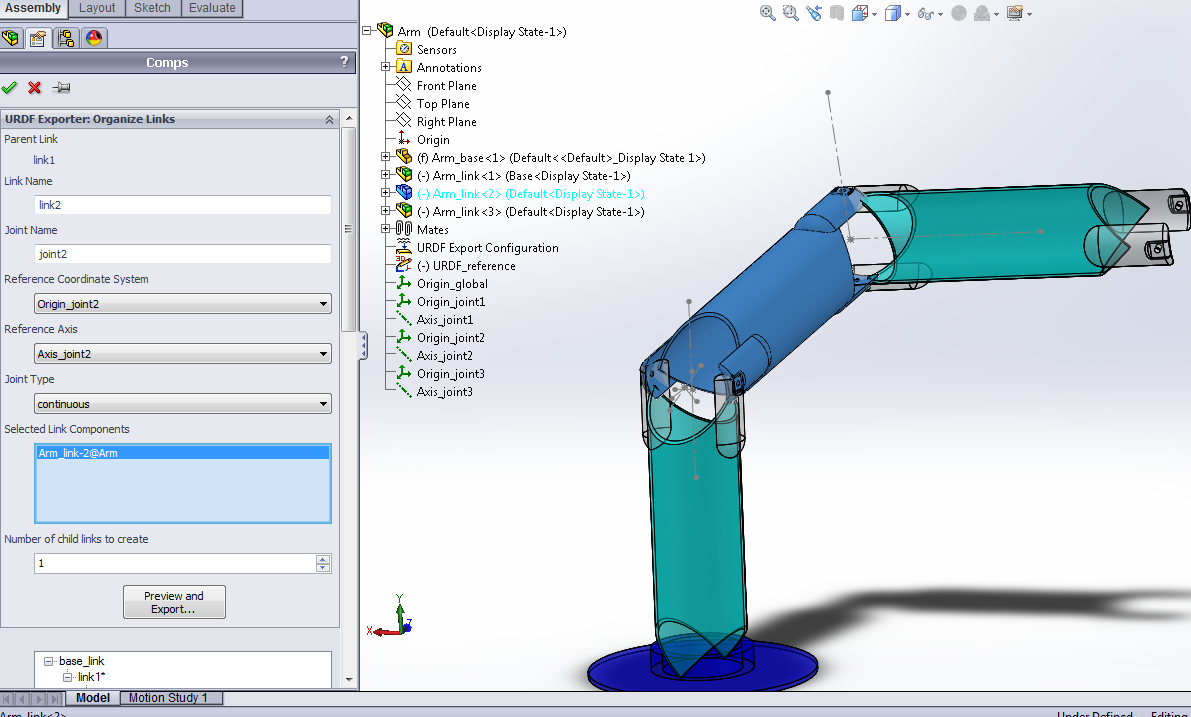
\includegraphics[width=\textwidth]{images/ExportPropertyManager}

For each link, you need to give it a unique name, give it a unique joint name, select the components (assemblies or parts) in SolidWorks that are to be associated with that link and add the necessary number of children. If you have reference coordinate systems or axes you would rather the tool to use, you may select those from the list. You can also manually specify what each joint type is. \emph{Both your custom reference coordinate systems and manual joint types are highly recommended so the user maintains control over the orientation of the child axes.} Each URDF has only one base link. The joint configurations are disabled for this one link because there doesn't exist a joint to a higher level link. You only need to name the link (if you don't want to call it base\_link), select its components and create its child links. 

In SolidWorks, if you select components on the actual assembly display instead of the FeatureManager Design Tree, you will only be able to select parts. More likely you would rather select assemblies that represent the entire link, in which case you will have select them from the Design Tree as pictured above. 

\emph{You can select multiple parts and assemblies for each resulting link in the URDF.  Any parts selected for one link will get welded together, and the resultant meshes and mass/inertia properties will be exported as if all included parts were one rigid body in the configuration they are placed in when the tool is run.}

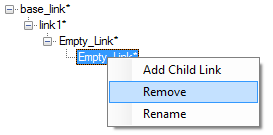
\includegraphics{images/ExportConfigTree}

The configuration tree shows you all the links you've added. For each child link on the tree, a joint will be created to its parent link. You can select any link you've already added to change its properties. Right clicking a link will allow you to add children to or remove the link. You can also drag and drop links to re-order them. Dragging a parent link onto a child will cause the child link to switch positions with the parent link. The parent link's other children still stay with the original parent link. 

Clicking the green check mark will just save your configuration and exit. Clicking the red x will allow you to exit without saving changes made to your configuration. 

When you are ready to build your URDF, click ``Preview and Export\ldots''. If you have specified the tool to automatically generate coordinate systems or axes, it will build them at this stage. 

\subsection{Joint Properties}
\indent Should you find that these joint origins are often not created in the most desirable location, you can change the reference coordinate systems and axes to suit your needs outside of the exporter. However, the model will work fine built as-is. The 3D Sketch is just used for temporary construction, but you may find it useful for adjusting the locations of the reference geometry. Pressing cancel on the Joint Properties page will allow you to save the names of the coordinate systems and axes to your configuration. You may then proceed to adjust the coordinate systems and axes. Restart the export process by clicking ``File\verb|>| Export to URDF''. Ensure that the right names of coordinate systems and axes are saved for each link. The tool will no longer build them and instead refer to the reference geometry already in place. 

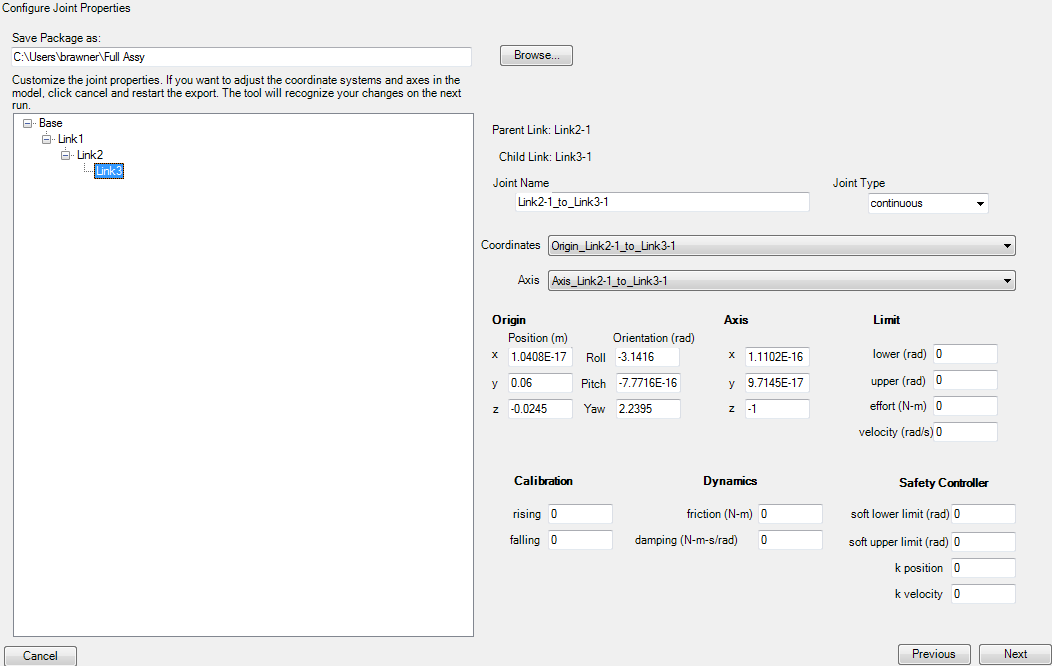
\includegraphics[width=\textwidth]{images/ExportJointProperties}

The joint page includes a non-configurable joint tree, where clicking each joint will bring up its properties on the right-hand side. You can customize the properties of any joint before exporting.  These properties will not be saved however with the configuration. They will need to be re-entered each time.

\emph{Special care should be taken with the sign of the axis of rotation.  Typically these should be positive numbers to obey the right-hand rule, especially if you defined your own coordinate reference geometries.  Numbers for both positions and axes that are close to zero ($\sim10^{-15}$) can be zeroed without consequence.}

Fields that are initially blank are not required by the URDF specifications. If they are left blank they will not be written to the URDF file. If you change a property of a section that includes other required fields, but neglect to specify them, they will be filled in with 0.

\subsection{Link Properties}
\indent This page presents a similar view to the Part Exporter discussed earlier. You can change the link properties of any link in your tree. You can add a texture, change the color, change the origins of different sections, change the moment of inertia tensor, mass, etc. These changes will also not be saved with your configuration. \emph{Varying colors can be useful for visually identifying separate links or degrees of freedom later on.  If you input the mass properties into your Solidworks files, it is recommended to leave all the inertial properties alone.}

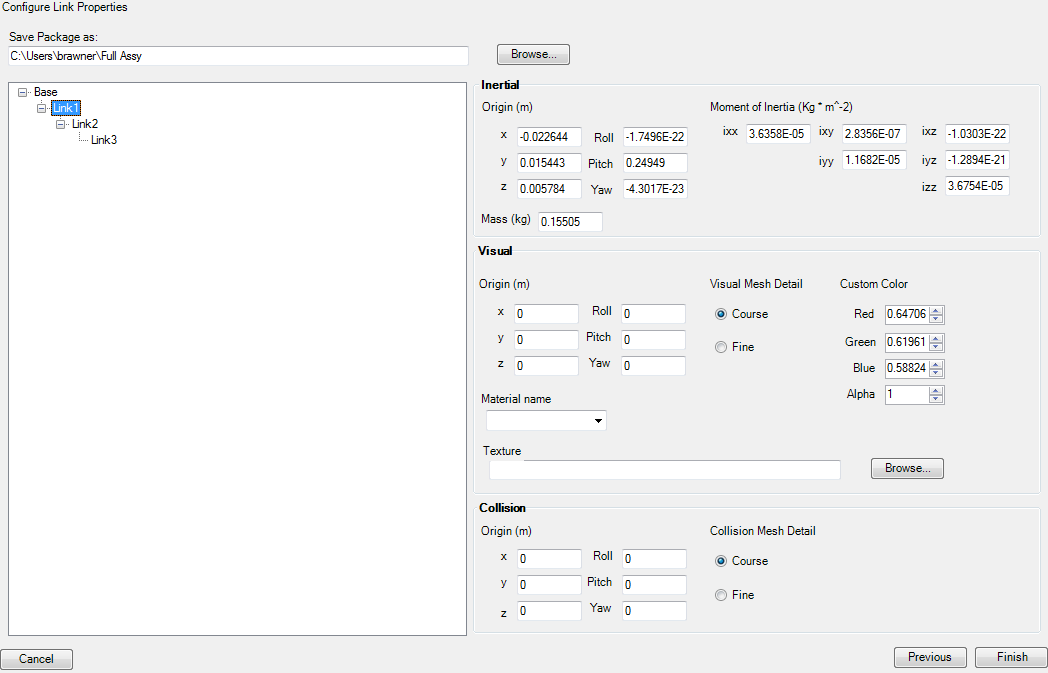
\includegraphics[width=\textwidth]{images/ExportLinkProperties}

Click Finish to create your URDF package.

\subsection{The built package}\label{sec:ExportBuiltPackage}
\indent The package will contain directories for meshes, textures and robots. 
\textit{
For \drake, you only need the .STL files in the meshes folder and the URDF in the robots folder.  These files require a little bit of manual work before they can be used by \drake.  The .STL files need to be converted into .obj files using a program like Meshlab.  After conversion, the \mcode{<visual>} tags in the URDF need to be changed from their ROS declaration to the appropriate .obj filenames.  \\ \indent Also it is a good idea to simplify the \mcode{<collision>} geometry using primitives rather than the default meshes.  Refer to the URDF documentation for the different options available for collision references.
} 
If you find that your meshes are too complicated you can refer to \autoref{sec:ExportTips} or you can simplify complicated meshes by using a program like MeshLab or Blender. 
\\

Except where otherwise noted, the ROS wiki is licensed under Creative Commons Attribution 3.0.

\section{How to organize a complicated SolidWorks assembly for export}\label{sec:ExportTips}
\textbf{Description:} This tutorial covers how to organize your SolidWorks assembly to create a better workflow and also how to reduce the exported mesh complexity when dealing with complicated assemblies.
\\

\noindent \textbf{Tutorial Level:} BEGINNER
\subsection{Introduction}
\noindent This tutorial is a collection of all techniques I can think of to help make the exporting process simpler.
 
\noindent Goals in simplification: 
\begin{enumerate}
\item Keep work flow as natural as possible and integrate easily with project 
\item Reduce mesh complexity without sacrificing goal \#1 
\end{enumerate}

\subsection{Assemble all link components into one assembly}
The easiest way to organize your assembly is to have as few components as possible associated with each link. Instead, group as much as possible into a single assembly for every independent link. This suggestion is not due to limitations in the software, but instead it's more likely with a longer list that the associated components will change throughout the development process. So this practice will reduce the amount of configuration necessary before each export. It will also help ensure that the saved export configuration will remain up-to-date for everyone who opens the assembly. 

Obviously this won't help if you suddenly decide your robot arm requires 6 degrees of freedom instead of 5, but as you add more components to it it should minimize tinkering around with the configuration.

\subsection{Home State Mates (a.k.a setting the zero position)}\label{sec:ExportHomeState}
\emph{The exporter will use the reference geometry coordinate systems you specify for the resulting URDF model.  If these are tied to the child link, then setting the child link in a proper orientation before doing an export is critical to making your zero positions correct.  For this case, it is recommended to maintain mates for each degree of freedom.} Name these mates something recognizable (like `Shoulder Home State') so that it is a simple manner of suppressing them for the first export process. Once the reference geometries for the joints have been created and the joint type has been saved, then you do not need to suppress the mates each time. The tool will refer to its configuration instead of trying to automatically generate them, which would be inhibited anyway by the unsuppressed home state mates. However, you should ensure the coordinate systems and axes are located properly, and their names are saved within the configuration. 

\subsection{Setup Configurations and Display States}
To avoid exporting the meshes of every single nut, bolt, screw, or flux capacitor in your assembly, you can hide them before exporting. However, solely hiding them doesn't allow you to save this configuration for later exports. 
Create a Display State specifically for exporting. Click the configuration tab in the Property Manager and right click the bottom section where Display States are located. Add a new display state and name it something like ``URDF Export'' so that you and others can return to it later. From the property manager tree, hide all the subassemblies and parts you do not want displayed. Double clicking the original display state, probably `Display State-1', unhides all the components that are hidden in the URDF Export display state. 
Most SolidWorks users are familiar with Configurations, but these only allow you to suppress components or features. This is not useful because the exporter will ignore all those components when calculating mass properties and your mates may break. Display States is the analogous feature but for hiding parts. 
SolidWorks allows you to `Link Display States to Configuration', but this is not recommended. Despite the ability to link configurations in the main assembly with configurations in subassemblies, the Display States aren't inherited for some reason. So you'll have to bite the bullet and work in the top level assembly to hide all the subassembly components. Annoying I know, and it's SW's bug, not mine. I'm open to suggestions for how to deal with this. 

\subsection{Skin Parts}
SolidWorks does not have great tools for reducing the triangle count in a mesh below their `course' export option, which is never course enough for simulation/collision detection. Therefore when not using the Exporter, many are forced to create their own skin meshes and incorporate them into the URDF. Since our goal is to eliminate work outside of the natural work flow specifically for exporting, it's recommended to create your skin part in SolidWorks. 
Create a part that envelopes your entire link and that vaguely resembles its shape. Set the material on this skin part to `Air'. It won't matter, but you might want to change the appearance. Insert it into your main assembly. Place this component over your link in the approximate location and create a `lock' mate to another component in your assembly. Then activate your `URDF Export' Display State and hide every component but your skin parts. Then in your default `Display State-1' or whatever its called, hide the skin parts. 
\\
\\
Except where otherwise noted, the ROS wiki is licensed under Creative Commons Attribution 3.0.